\documentclass{article}

%Header Dimensions
%https://tex.stackexchange.com/questions/40183/problem-with-the-header-footer-width#40184
\usepackage[margin=0.5in,bottom=0.5in,top=0.5in]{geometry}

%Package required for empty set
\usepackage{amssymb}

%Package required for Comb/Perm symbol and matrices
\usepackage{amsmath}

%Package for graphics
\usepackage{graphicx}

%Package for placing graphics
\usepackage{float}

%Places box around graphics
% Uncomment to box 
% \floatstyle{boxed} 
% \restylefloat{figure}


%For inserting code
\usepackage{listings}
%https://www.sharelatex.com/learn/Code_listing

\begin{document}

	
%%%%%%%%%%%%%%%%%
%CUSTOM COMMANDS%
%%%%%%%%%%%%%%%%%

	%This line surpresses the page number
%https://tex.stackexchange.com/questions/7355/how-to-suppress-page-number
\thispagestyle{empty}

%Make empty set pretty
% https://tex.stackexchange.com/questions/22798/nice-looking-empty-setup
\let\oldemptyset\emptyset
\let\emptyset\varnothing


%Combinatorial notation
%From https://tex.stackexchange.com/questions/107125/is-there-a-command-to-write-the-form-of-a-combination-or-permutation
\newcommand*{\Perm}[2]{{}^{#1}\!P_{#2}}
\newcommand*{\Comb}[2]{{}_{#1}C_{#2}}


	
\textbf{	Matt Fletcher CS317-02 Homework 1}
\smallskip


1.  


\begin{figure}[H]
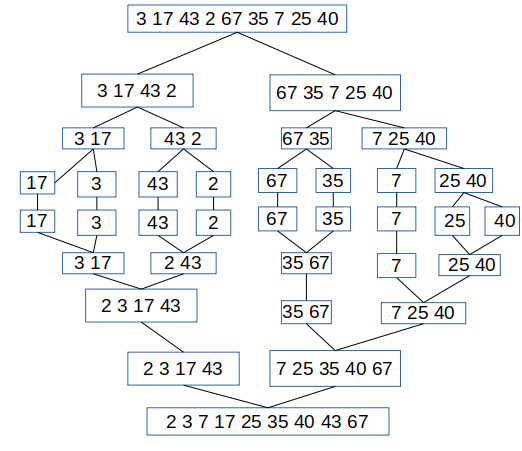
\includegraphics[scale=0.5]{./P1/sorted}
\centering
\end{figure}

\noindent\rule{8cm}{0.4pt}



2. 

Three steps:

a) Move R to left, and L to R until $R<P$ and $L>P$. 

b) If during (a) R and L did not cross, swap R and L, and continue (a). 

c). If during (a) R and L did cross, swap R and P, freeze P in its new place, split the list in 2 around P, and recursively continue (a) on each new list. 

An asterisk next to an element indicates that it is frozen. 

\begin{lstlisting}
P 	L 							R
43	21	90	8	44	35	6	2	13

P 		L 						R
43	21	90	8	44	35	6	2	13

P 		R 						L
43	21	13	8	44	35	6	2	90

P 		L 						R
43	21	13	8	44	35	6	2	90

P 		 		L			R	
43	21	13	8	44	35	6	2	90

P 		 		L			R	
43	21	13	8	2	35	6	44	90

P 		 				R	L	
43	21	13	8	2	35	6	44	90

R 		 				P	L	
6	21	13	8	2	35	43	44	90

P	L	 			R		PL	R
6	21	13	8	2	35	43*	44	90

P	L	 		R			PR	L
6	21	13	8	2	35	43*	44	90

P	R	L 						
6	2	13	8	21	35	43*	44*	90

		P 	L		R			
2	6*	13	8	21	35	43*	44*	90

		P 	R	L				
2	6*	13	8	21	35	43*	44*	90

		 		PL	R			
2	6*	8	13*	21	35	43*	44*	90

		 		PR	L			
2	6*	8	13*	21	35	43*	44*	90

		 						
2	6*	8	13*	21*	35	43*	44*	90

\end{lstlisting}

All elements are either frozen or single element lists, therefore, the list is sorted. 

\noindent\rule{8cm}{0.4pt}

3. 

Five applications of graph theory: social media connections, navigation, cellular connections to towers, circuit design, register allocation

\noindent\rule{8cm}{0.4pt}


4. 
A directed graph has edges which indicate the direction they travel. The direction of travel cannot oppose the node. On the other hand, an undirected graph allows travel both ways along any edge. 

\noindent\rule{8cm}{0.4pt}

5. 

a) Edges: ac, cf, ab, be, bd
	
	Nodes:a,b,c,d,e,f

b) Edges: fc, ca, ba, be, bd
	
	Nodes:  a,c,f,b,e,d


\noindent\rule{8cm}{0.4pt}

6. 

a) Adjacency List

\begin{lstlisting}
[ a ]-->[ b ]-->[ c ]-->[ d ]-->[ e ]-->[ f ]-->[ g ]
 |       |       |       |       |       |       | 
 v       v       v       v       v       v       v
[->b]   [->d]   [->f]   [->b]   [->b]   [->c]   [->e]
 |       |       |       |       |       |       | 
 v       v       v       v       v       v       v
[->c]   [->e]   [->a]   [->0]   [->g]   [->g]   [->f]
 |       |       |               |       |       | 
 v       v       v               v       v       v
[->0]   [->a]   [->0]           [->0]   [->0]   [->0]
         |
         v
        [->0] 
\end{lstlisting}


a) Adjacency Matrix

\begin{table}[H]
\begin{tabular}{l|l|l|l|l|l|l|l|}
\cline{2-8}
 & A & B & C & D & E & F & G \\ \hline
\multicolumn{1}{|l|}{A} & 0 & 1 & 1 & 0 & 0 & 0 & 0 \\ \hline
\multicolumn{1}{|l|}{B} & 1 & 0 & 0 & 1 & 1 & 0 & 0 \\ \hline
\multicolumn{1}{|l|}{C} & 1 & 0 & 0 & 0 & 0 & 1 & 0 \\ \hline
\multicolumn{1}{|l|}{D} & 0 & 1 & 0 & 0 & 0 & 0 & 0 \\ \hline
\multicolumn{1}{|l|}{E} & 0 & 1 & 0 & 0 & 0 & 0 & 1 \\ \hline
\multicolumn{1}{|l|}{F} & 0 & 0 & 1 & 0 & 0 & 0 & 1 \\ \hline
\multicolumn{1}{|l|}{G} & 0 & 0 & 0 & 0 & 1 & 1 & 0 \\ \hline
\end{tabular}
\end{table}


b) Adjacency List

\begin{lstlisting}
[ a ]-->[ b ]-->[ c ]-->[ d ]-->[ e ]-->[ f ]-->[ g ]
 |       |       |       |       |       |       | 
 v       v       v       v       v       v       v
[->b]   [->d]   [->a]   [->0]   [->0]   [->c]   [->0]
 |       |       |                       |     
 v       v       v                       v    
[->g]   [->e]   [->0]                   [->g]
 |       |                               |  
 v       v                               v   
[->0]   [->0]                           [->0]

\end{lstlisting}

b) Adjacency Matrix

\begin{table}[H]
\begin{tabular}{l|l|l|l|l|l|l|l|}
\cline{2-8}
 & A & B & C & D & E & F & G \\ \hline
\multicolumn{1}{|l|}{A} & 0 & 1 & 0 & 0 & 0 & 0 & 1 \\ \hline
\multicolumn{1}{|l|}{B} & 0 & 0 & 0 & 1 & 1 & 0 & 0 \\ \hline
\multicolumn{1}{|l|}{C} & 1 & 0 & 0 & 0 & 0 & 0 & 0 \\ \hline
\multicolumn{1}{|l|}{D} & 0 & 0 & 0 & 0 & 0 & 0 & 0 \\ \hline
\multicolumn{1}{|l|}{E} & 0 & 0 & 0 & 0 & 0 & 0 & 0 \\ \hline
\multicolumn{1}{|l|}{F} & 0 & 0 & 1 & 0 & 0 & 0 & 1 \\ \hline
\multicolumn{1}{|l|}{G} & 0 & 0 & 0 & 0 & 0 & 0 & 0 \\ \hline
\end{tabular}
\end{table}

\noindent\rule{8cm}{0.4pt}


7.  Traversal order:

A 1/16

B 2/9

C 10/15

D 3/4

E 5/8

F 11/14

G 12/13

Stack order:

Top $\rightarrow$$\rightarrow$$\rightarrow$ $\rightarrow$Bottom

$\boxed{G F C H E D B A}$

\noindent\rule{8cm}{0.4pt}


8.  Traversal order:

A 1

B 2

C 2

D 3

E 3 

F 4

G 5

Queue:

Front $\rightarrow$$\rightarrow$$\rightarrow$ $\rightarrow$Back

$\boxed{A B C D E F G}$

\noindent\rule{8cm}{0.4pt}


9.  

Efficiency of Matrix: $\Theta(\|V^2\|)$

Efficiency of List: $\Theta(\|V\|+  \|E\|)$

\noindent\rule{8cm}{0.4pt}


10. The greedy technique builds a solution piece by piece by picking the most obvious benefit first, without ever reconsidering a decision. It generates a globally optimal solution from a locally optimized choice. 

TODO Greedy algorithm and the greedy choice property. 


\noindent\rule{8cm}{0.4pt}

11. A spanning tree is a set of edges that connects every node in the graph without forming loops or cycles. 


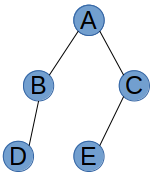
\includegraphics[scale=0.5]{./P11/1}
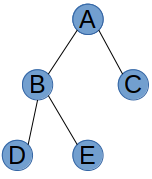
\includegraphics[scale=0.5]{./P11/2}
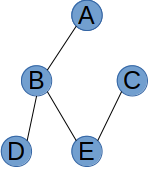
\includegraphics[scale=0.5]{./P11/3}
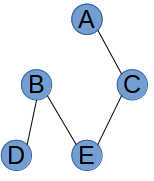
\includegraphics[scale=0.5]{./P11/4}
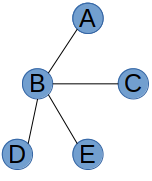
\includegraphics[scale=0.5]{./P11/5}
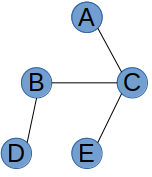
\includegraphics[scale=0.5]{./P11/6}
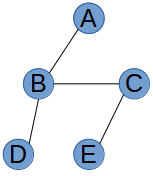
\includegraphics[scale=0.5]{./P11/7}


TODO FIND ALL SPANNING TREES. 

\noindent\rule{8cm}{0.4pt}

12. A minimum spanning tree (MST) is the smallest tree that connects every node in the graph. If the graph is weighted, the smallest tree has the smallest sum of weights. If the graph is unweighted, the MST has the smallest number of edges. 

An example of a minimum spanning tree is determining the minimum amount of wire needed to connect multiple nodes. 

\noindent\rule{8cm}{0.4pt}

13. 

Kruskal's Algorithm: 

$\rightarrow$1. Create a table with each edge sorted in ascending order. 
\begin{table}[H]
\begin{tabular}{|l|l|l|l|l|l|l|l|l|l|l|}
\hline
Edge & CD & DE & AD & AE & BC & AB & BE & BD & AC & BC \\ \hline
Weight & 1 & 2 & 3 & 4 & 5 & 6 & 6 & 8 & 9 & 11 \\ \hline
\end{tabular}
\end{table}


$\rightarrow$2. Starting from either node on the smallest line, attach the next smallest line that does not create a loop. 

Start by attaching line $CD$, weight 1. 

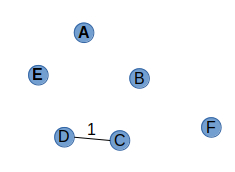
\includegraphics[scale=0.5]{./P13/kruskals/1}

Then, find the smallest weighted edge from any end node that does not create a cycle. This is edge DE. 

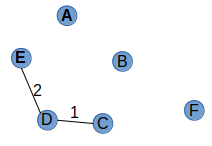
\includegraphics[scale=0.5]{./P13/kruskals/2}

Same as before, add edge AD. 

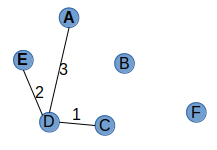
\includegraphics[scale=0.5]{./P13/kruskals/3}

Although AE is the next smallest edge, adding it would create a cycle. So we add BC instead. 

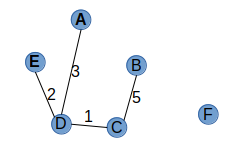
\includegraphics[scale=0.5]{./P13/kruskals/4}

Add the next edge. 

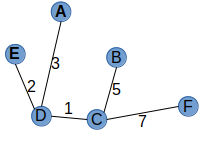
\includegraphics[scale=0.5]{./P13/kruskals/5}

At this point, all the nodes are connected and adding any more lines would result in a cycle being created. Hence, we are done. 


TODO EXPLAIN PRIMS ALGORITHM

Prims algorithm starts from some vertex (Vertex A in this example) and finds the smallest addition that can be added to the current tree in order to not create a cycle. 

A dashed line indicated that edge has been selected. 

Start at vertex A. There are 4 edges that can be selected: AE, AD, AC, and AB. AE has the lowest weight, so we select that edge. 

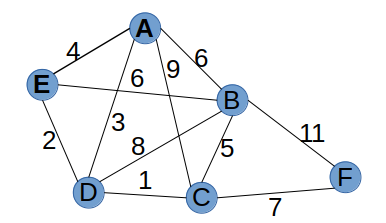
\includegraphics[scale=0.5]{./P13/prims/0}

Now, we check all of the edges coming out of both vertex A and E. The lowest weight gets selected, and we choose edge ED. 

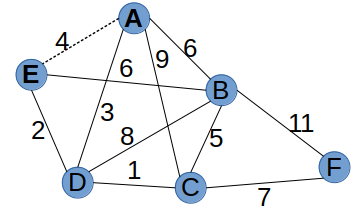
\includegraphics[scale=0.5]{./P13/prims/1}

At this point, we check vertices A, E, and D. Although DA has the lowest weight, it would cause a cycle. So, we skip it and check the other edges. 

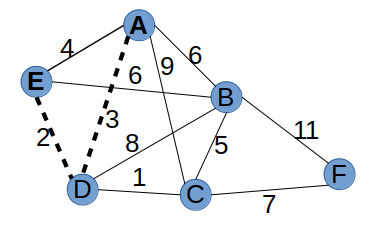
\includegraphics[scale=0.5]{./P13/prims/2}

Continuing...

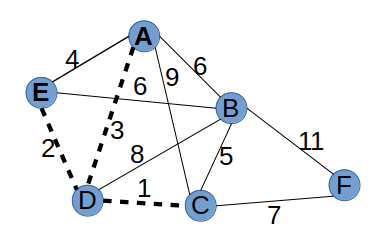
\includegraphics[scale=0.5]{./P13/prims/3}

Almost there...

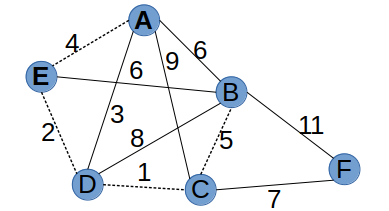
\includegraphics[scale=0.5]{./P13/prims/4}


And done!

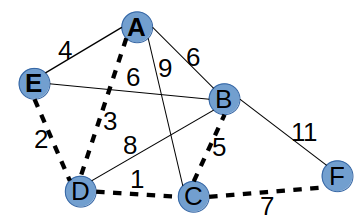
\includegraphics[scale=0.5]{./P13/prims/5}


We are done because all vertices have been reached, and no loops or cycles have been created. The total weight is $4+2+1+5+7=\boxed{19}$.






\noindent\rule{8cm}{0.4pt}

14. 

\noindent\rule{8cm}{0.4pt}


15.  

\noindent\rule{8cm}{0.4pt}

16. 


\noindent\rule{8cm}{0.4pt}

\end{document}
